\documentclass[11pt,a4paper]{amsart}

\usepackage{amsmath, amssymb}
\usepackage{dsfont}
\usepackage[dutch]{babel}
\usepackage{geometry}
\usepackage{commath}
\usepackage{url}
\usepackage{enumerate}
\usepackage{graphicx}
\usepackage{mathtools}
\usepackage{todonotes}
%\setlength{\parindent}{0pt}
\geometry{%
  includeheadfoot,
  margin=2cm
}

\newtheorem*{problem}{Problem}
\newtheorem*{lemma}{Lemma}
\theoremstyle{definition}
\newtheorem*{answer}{Answer}

\newcommand{\bbone}{\mathds{1}}
\DeclareMathOperator*{\diam}{diam}
\DeclareMathOperator*{\spann}{span}
\DeclareMathOperator*{\init}{init}
\DeclareMathOperator*{\ext}{ext}
\newcommand{\udlrarrow}{\mathrlap{\,{\scriptscriptstyle \updownarrow}}{\scriptscriptstyle \leftrightarrow}}

%\input{/Users/janwesterdiep/Dropbox/Commands.tex}
\newcommand{\T}{{\mathcal T}}
\newcommand{\R}{\mathbb{R}}

\begin{document}

\title{Eerste implementatie blauwe tekstje, \today}
\author{Jan Westerdiep}
\maketitle

Gegeven is een initial matching conforming triangulatie $\T_0$. We gaan hier
vertices in toevoegen door driehoeken te verfijnen volgens nvb. We willen, gegeven
een lokaal verfijnde triangulatie $\T \geq \T_0$, \emph{snel} een matvec
$a_2(\Psi_{\text{hb}}, \Psi_{\text{hb}}) \vec v$ uit kunnen rekenen voor
$\Psi_{\text{hb}}$ de hierarchische basis wrt vertices van $\T$. Dit kan in
$\mathcal O(\# \T)$ operaties, waarbij $\# \T$ het aantal vertices in $\T$ is.
Hiertoe zullen we gebruik maken van de single-scale basis $\Phi_{\text{ss}}$ op
$\T$.

\section*{De \texttt{Vertex} klasse}
We hebben een klasse \texttt{Vertex}, met attributen
\begin{description}
  \item[x, y] de $x$- en $y$-coordinaten van de vertex;
  \item[on\_bdr] of de vertex op de domain boundary ligt.
\end{description}

\section*{De \texttt{Triangle} klasse}
We hebben een klasse \texttt{Triangle}, met attributen
\begin{description}
  \item[idx] de index in de \texttt{Triangulation.tris}-array;
  \item[vertex\_ids] de indices van de drie hoekpunten in de \texttt{Triangulation.verts}-array;
  \item[parent] een reference/pointer naar de parent van deze driehoek (mogelijk \texttt{None});
  \item[children] twee pointers naar de kinderen van deze driehoek (mogelijk \texttt{None});
  \item[nbrs] een 3-tuple van pointers naar onze buren. Nbr $0$ zit \emph{tegenover} vertex 0, etc;
  \item[area] de area van deze driehoek.
\end{description}
Deze klasse heeft een paar convenience-methodes:
\begin{description}
  \item[edge(i)] returned \texttt{[self.vertex\_ids[(i + 1) \% 3], self.vertex\_ids[(i + 2) \% 3]]};
  \item[is\_leaf()] returned \texttt{not len(self.children)}.
\end{description}

\section*{De \texttt{Triangulation} klasse}
Als laatste de klasse \texttt{Triangulation}, met attributen
\begin{description}
  \item[verts] een array van \texttt{Vertex}-objecten;
  \item[tris] een array van \texttt{Triangle}-objecten;
  \item[root\_ids] een \texttt{set} met de indices van driehoeken met generatie 0;
  \item[history] array 2-tupels \texttt{(new\_vertex\_id, bisected\_triangle)} welke we zo omschrijven.
\end{description}
Deze klasse heeft twee methodes voor het initialiseren en refinen:
\begin{description}
  \item[init(verts, tris)] initialiseert $\T$ en de \texttt{Triangle}- en
    \texttt{Vertex}-attributen (\texttt{nbrs} resp.~ \texttt{on\_bdr});
  \item[refine(tri)] maakt een conforming refinement waarin \texttt{tri} gerefined is. Psuedocode:
\begin{verbatim}
  als tri geen leaf is: return # deze driehoek is al ge-refined.
  nbr = tri.nbrs[0]
  if nbr == None:  # we zitten aan de rand van het domein.
    self.bisect(tri)
  else if nbr.edge(0) tegenover tri.edge(0):  # shared refinement edge.
    self.bisect_pair(tri, nbr)
  else:
    self.refine(nbr)
    self.bisect_pair(tri, het kind van nbr grenzend aan tri.edge(0))
\end{verbatim}
\end{description}
De \texttt{refine}-methode maakt gebruik van de volgende \emph{private} methodes.
Wij zorgen dat deze slechts aangeroepen worden wanneer het mag (om conformiteit van de triangulatie te bewaren).
\begin{description}
  \item[bisect(tri, new\_vertex\_id=None)] doet NVB van de gegeven driehoek. Pseudocode:
\begin{verbatim}
  als new_vertex_id == None:
    bouw object new_vertex en plaats in de self.verts array
    plaats (new_vertex_id, tri.idx) achteraan in de self.history array
  bouw de kinderen C1, C2 van tri en plaats in de self.tris array
  C1.nbrs = [tri.nbrs[2], None, C2]; C2.nbrs = [tri.nbrs[1], C1, None]
  vervang tri door C1 in tri.nbrs[2], door C2 in tri.nbrs[1]
  return C1, C2
\end{verbatim}
  \item[bisect\_pair(T1, T2)] bisect \texttt{T1} en \texttt{T2}, en zet alle neighbour-info goed.
\end{description}

Met deze basis kunnen we gemakkelijk twee methodes bouwen:
\begin{description}
  \item[applyT(v)] pakt een vector $\vec v \in \R^{\# \T}$ coefficienten en geeft de vector $\vec w \in \R^{\# \T}$ zdd $\Psi_{\text{hb}}^\top \vec v = \Phi_{\text{ss}}^\top \vec w$,
    i.e.,~\texttt{applyT(v)} applied de hierarchic-to-singlescale operator.
    Pseudocode:
\begin{verbatim}
  w = v
  for (vi, Ti) in self.history:
    godfathers = self.tris[Ti].edge(0)
    w[vi] += w[godfathers[0]]/2 + w[godfathers[1]]/2
  return w
\end{verbatim}
  \item[applyT\_transpose(v)] applies de getransponeerde, met pseudocode
\begin{verbatim}
  w = v
  for (vi, Ti) in reversed(self.history):  # NB: in reversed order
    godfathers = self.tris[Ti].edge(0)
    w[godfathers[0]] += w[vi]/2
    w[godfathers[1]] += w[vi]/2
  return w
\end{verbatim}
  \item[apply\_HB\_*(v)] hebben voor $* \in \set{\mathtt{mass}, \mathtt{stiffness}}$ dan een simpele
    implementatie:
\begin{verbatim}
  return self.applyT_transpose(self.apply_SS_*(self.applyT(v)))
\end{verbatim}
\end{description}
Daarvoor is het wel zaak om de mass- en stiffness matrices snel te applyen. Dit kan door
\begin{description}
  \item[apply\_SS\_mass(v)] gaat in $\mathcal O(\# \mathtt{self.tris}) \eqsim \mathcal O(\# \T)$ operaties volgens
\begin{verbatim}
  elt_mass = 1/12 * [[2, 1, 1], [1, 2, 1], [1, 1, 2]]
  w = [0, ..., 0]
  for tri in self.tris:
    if not tri.is_leaf(): continue
    N = tri.vertex_ids
    for i in [0,1,2] en j in [0,1,2]:
      w[N[j]] += elt_mass[i,j] * tri.area * v[N[i]]
  return w
\end{verbatim}
  \item[apply\_SS\_stiffness(v)] gaat in dezelfde complexiteit. Ik vond dit in een paper:
\begin{verbatim}
  w = [0, ..., 0]
  for tri in self.tris:
    if not tri.is_leaf(): continue
    N = tri.vertex_ids
    V = [self.verts[ni] for ni in N]
    D = [[V[2].x - V[1].x, V[0].x - V[2].x, V[1].x - V[0].x],
         [V[2].y - V[1].y, V[0].y - V[2].y, V[1].y - V[0].y]]
    elt_stiff = matmat(D.T, D) / (4 * tri.area)
    for i in [0,1,2] en j in [0,1,2]:
      w[N[j]] += elt_stiff[i,j] * v[N[i]]
  return w
\end{verbatim}
\end{description}

\section*{Test hierarchic-to-singlescale implementatie}
Ik kan niet zo 1-2-3 echt netjes laten zien dat wat ik doe, het juiste is. Maar
het kwam er wel heel snel uitrollen toen ik op papier een beetje voorbeelden uit
ging werken. De methode \texttt{applyT()} is geen recursie, en stom genoeg kon ik
ook niet helemaal zien hoe je hem als recursie kon opschrijven.

\subsection*{Wat obvious tests}
Ik heb een paar obvious dingen getest, en die komen er allemaal positief uit:
\begin{itemize}
  \item is \texttt{applyT(v + a*w) == applyT(v) + a applyT(w)} voor een paar willekeurige $\vec v, a, \vec w$?
  \item is \texttt{< applyT(v), z > == <v, applyT\_transpose(z) >} voor een paar willekeurige $\vec v, \vec z$?
  \item is \texttt{vertex.on\_bdr} correct voor willekeurige vertices op een verfijnde square?
\end{itemize}

\subsection*{Een FE-oplossing}
De laatste test was om de vergelijking $- \triangle u = \bbone, u = 0$ op te lossen op $[-1,1]^2$.
In \url{http://people.inf.ethz.ch/arbenz/FEM17/pdfs/0-19-852868-X.pdf} staat
de oplossing uitgeschreven als oneindige som (welke we tot eoa precisie uit
kunnen rekenen en op een aantal punten kunnen evalueren). Hiervoor hebben we
inderdaad alle onderdelen van onze implementatie nodig.

\subsubsection*{De right-hand side} Als eerste: we weten dat ons rechterlid voldoet aan
\[
  \langle \Psi_{\text{hb}}, \bbone\rangle = T^\top \langle \Phi_{\text{ss}}, \bbone\rangle =
  \mathtt{applyT\_transpose(apply\_SS\_mass}(\vec 1))
\]
waar $\vec 1$ een vector met allemaal enen is.

\subsubsection*{Een kleine shortcut voor nu}
Merk op dat de methodes die we tot nu toe hebben gebouwd, allemaal werken
\emph{op elke vertex}, en niet enkel op vertices in de domain interior. De
stiffness matrix die we op deze manier hebben gebouwd, is singulier. Ik heb er
voor nu voor gekozen om de boundary condities op te leggen door na elke call naar
\texttt{apply\_HB\_stiffness()}, alle waarden wrt rand-vertices op nul te zetten.
Dit heb ik ook gedaan voor de right-hand side.

\subsubsection*{De solver}
Ik heb de ingebouwde CG-solver van \texttt{scipy.sparse.linalg} gebruikt, welke
geen matrix nodig heeft, slechts een functie die een matvec doet.

\subsubsection*{De triangulatie}
We starten met een standaard initial triangulatie met 2 driehoeken. Vervolgens
doen we 9 uniform refinements, dwz 8 keer een lijst leaves genereren en
\texttt{refine(leaf)} aanroepen voor elke leaf. Omdat we op elke iteratie een
hierarchische basis hebben, kunnen we na elke uniform refinement een \texttt{rhs}-variabele
genereren (zoals hierboven) en testen dat de eerste zoveel waardes overeen komen
met de \texttt{rhs} uit de vorige iteratie.

\subsubsection*{De oplossing}
We krijgen een oplossing in hierarchical basis-coefficienten. Om deze oplossing
te testen tegen de uitgerekende reference solution, zullen we \texttt{sol\_SS = applyT(sol)}
gebruiken. We testen:
\begin{itemize}
  \item $|\mathtt{sol\_SS[4]} - u(0,0)| < 10^{-3}$ waarbij volgens Mathematica, $u(0,0) = 0.2946854131260553$;
  \item $|\mathtt{sol\_SS[i]} - u(\tfrac{1}{2},\tfrac{1}{2})| < 10^{-3}$ voor $i \in \set{9, 10, 11, 12}$ waarbij $u(\tfrac{1}{2},\tfrac{1}{2}) = 0.181145$;
\end{itemize}
Op deze manier ben ik er vrij van verzekerd dat deze methode een aardige oplossing
vindt. Een plot ziet er ook goed uit (de assen worden wat verschillend geplot maar maxima komen overeen).
\begin{figure}[b]
  \centering
  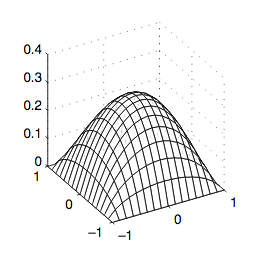
\includegraphics[width=0.3\linewidth]{img/paper-sol}
  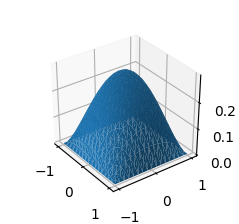
\includegraphics[width=0.3\linewidth]{img/fe-sol}
  \caption{Links: de oplossing uit het paper. Rechts: een plot van \texttt{sol\_SS}.}
\end{figure}
\clearpage

\subsection*{Een gekkigheidje}
We lopen niet level-voor-level door de vertices van de triangulatie. Zie de figuur
voor een illustratie. In de eerste figure zien we de progressie van de triangulaties
met de vertices genummerd. In de tweede figuur zie je de bijbehorende family-tree.
Een level-voor-level traversal zou gaan als
\[
  0 \to 1 \to 2 \to 3 \to 4 \to 5 \to 6 \to 8 \to 7
\]
whereas de \texttt{history}-array in ons geval een traversal geeft als
\[
  4 \to 5 \to 6 \to 7 \to 8.
\]
(Duidelijk worden in dit geval de roots van de family tree ook niet ge-traversed.)
Wel zijn beide traversals een \emph{topological ordering}, wat betekent dat een
kind pas aan bod komt wanneer beide parents al zijn geweest.

\begin{figure}[h!]
  \begin{tikzpicture}[scale=0.4]
    \draw (0,0) -- (4,0) -- (4,4) -- (0,4) -- (0,0); \draw (4,0) -- (0,4);
    \node[below left] at (0,0){0};
    \node[below right] at (4,0){1};
    \node[above right] at (4,4){2};
    \node[above left] at (0,4){3};
    \node[below] at (2,-1){$\T_0$};
  \end{tikzpicture}
  \hfill
  \begin{tikzpicture}[scale=0.4]
    \draw (0,0) -- (4,0) -- (4,4) -- (0,4) -- (0,0); \draw (4,0) -- (0,4);
    \node[below] at (2,-1){$\T_1$};

    \draw (0,0) -- (4,4); \node[right] at (2,2){4};
  \end{tikzpicture}
  \hfill
  \begin{tikzpicture}[scale=0.4]
    \draw (0,0) -- (4,0) -- (4,4) -- (0,4) -- (0,0); \draw (4,0) -- (0,4);
    \node[below] at (2,-1){$\T_2$};

    \draw (0,0) -- (4,4);
    \draw (2,2) -- (2,4); \node[above] at (2,4){5};
  \end{tikzpicture}
  \hfill
  \begin{tikzpicture}[scale=0.4]
    \draw (0,0) -- (4,0) -- (4,4) -- (0,4) -- (0,0); \draw (4,0) -- (0,4);
    \node[below] at (2,-1){$\T_3$};

    \draw (0,0) -- (4,4);
    \draw (2,2) -- (2,4);
    \draw (2,2) -- (0,2); \node[left] at (0,2){6};
  \end{tikzpicture}
  \hfill
  \begin{tikzpicture}[scale=0.4]
    \draw (0,0) -- (4,0) -- (4,4) -- (0,4) -- (0,0); \draw (4,0) -- (0,4);
    \node[below] at (2,-1){$\T_4$};

    \draw (0,0) -- (4,4);
    \draw (2,2) -- (2,4);
    \draw (2,2) -- (0,2);
    \draw (0,2) -- (2,4); \node at (1,3){7};
  \end{tikzpicture}
  \hfill
  \begin{tikzpicture}[scale=0.4]
    \draw (0,0) -- (4,0) -- (4,4) -- (0,4) -- (0,0); \draw (4,0) -- (0,4);
    \node[below] at (2,-1){$\T_5$};

    \draw (0,0) -- (4,4);
    \draw (2,2) -- (2,4);
    \draw (2,2) -- (0,2);
    \draw (0,2) -- (2,4);
    \draw (2,2) -- (2,0); \node[below] at (2,0){8};
  \end{tikzpicture}
  \caption{Een voorbeeldprogressie. We schrijven enkel de nieuwe vertex op per iteratie.}
\end{figure}
\begin{figure}
\end{figure}

\subsection*{Visuele check}
Als we de methode \texttt{applyT()} toepassen op de eenheidsvector $\vec v = e_i$
horende bij een hierarchische basisfunctie $\psi_i$, dan krijgen we de coefficienten
van $\psi_i$ in termen van de nodale/singlescale hoedfuncties $\Phi_{\text{ss}}$. In de derde figuur
zien we het resultaat, namelijk dat de code hierarchische basisfuncties inderdaad
terugvindt.
\begin{figure}
  \begin{minipage}{0.4\linewidth}
    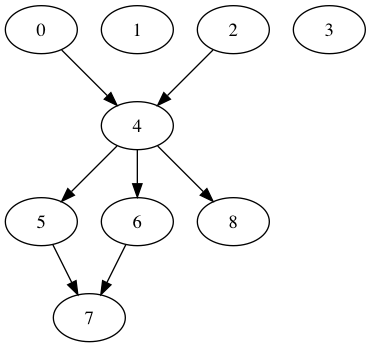
\includegraphics[width=\linewidth]{img/vertex-tree.png}
  \end{minipage}
  \begin{minipage}{0.55\linewidth}
    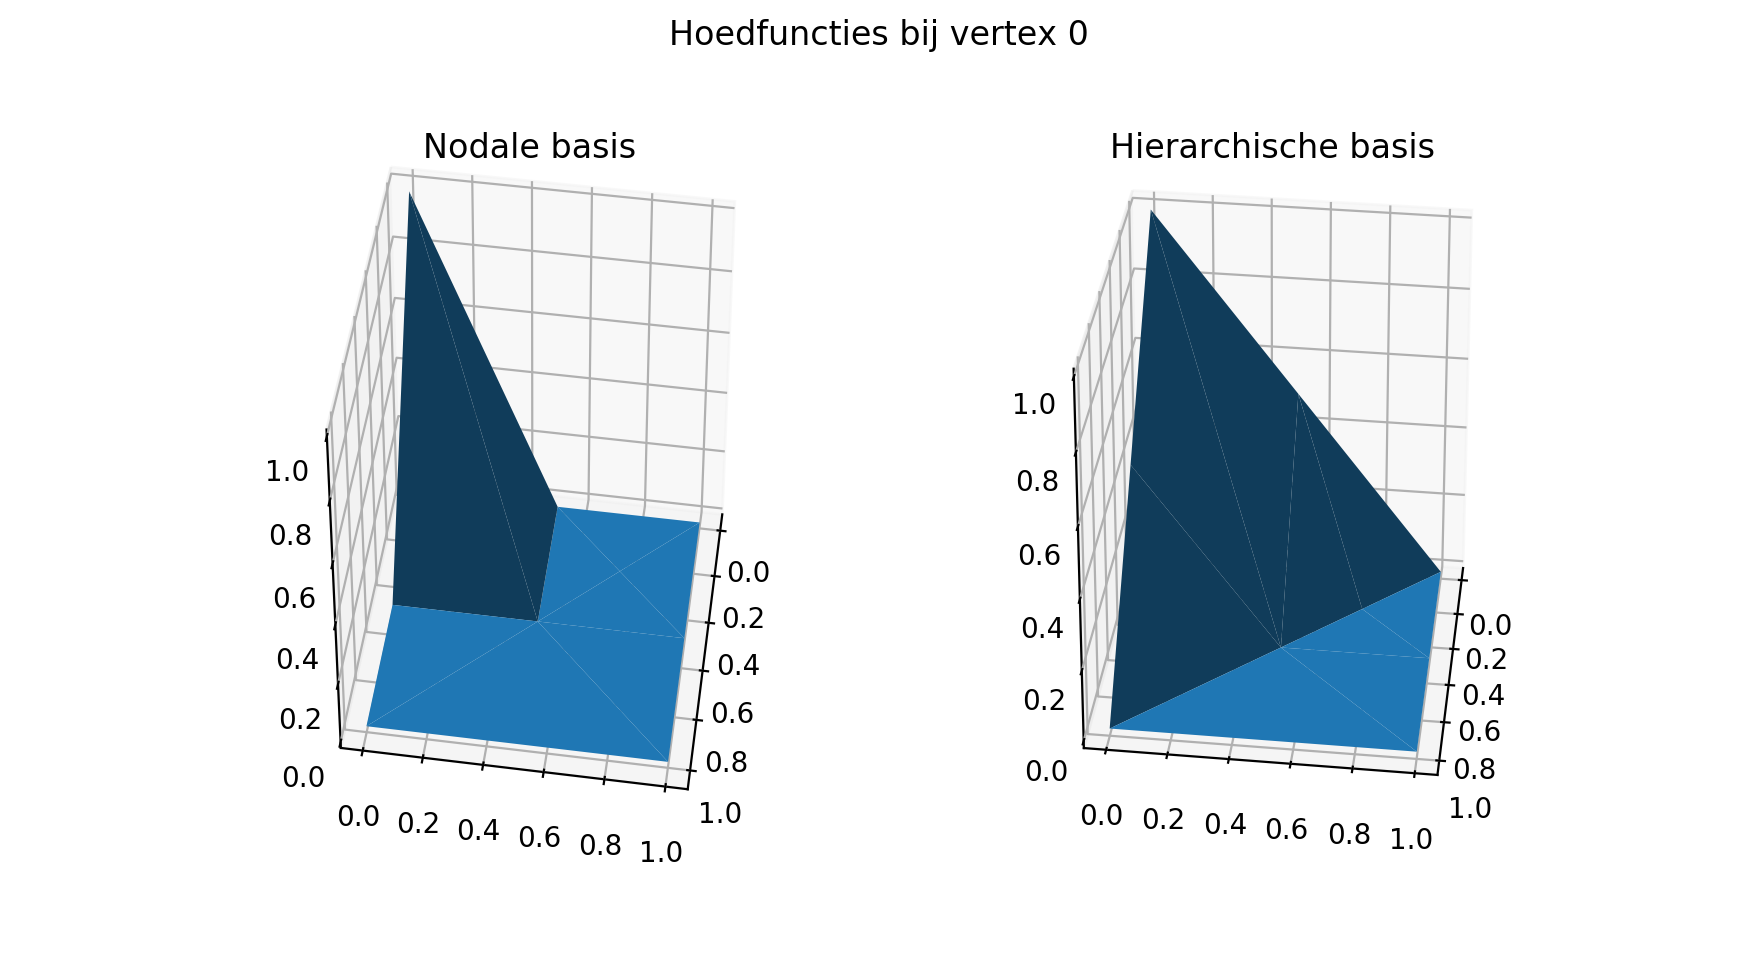
\includegraphics[width=\linewidth]{img/h0.png}\\
    \vspace{-1em}
    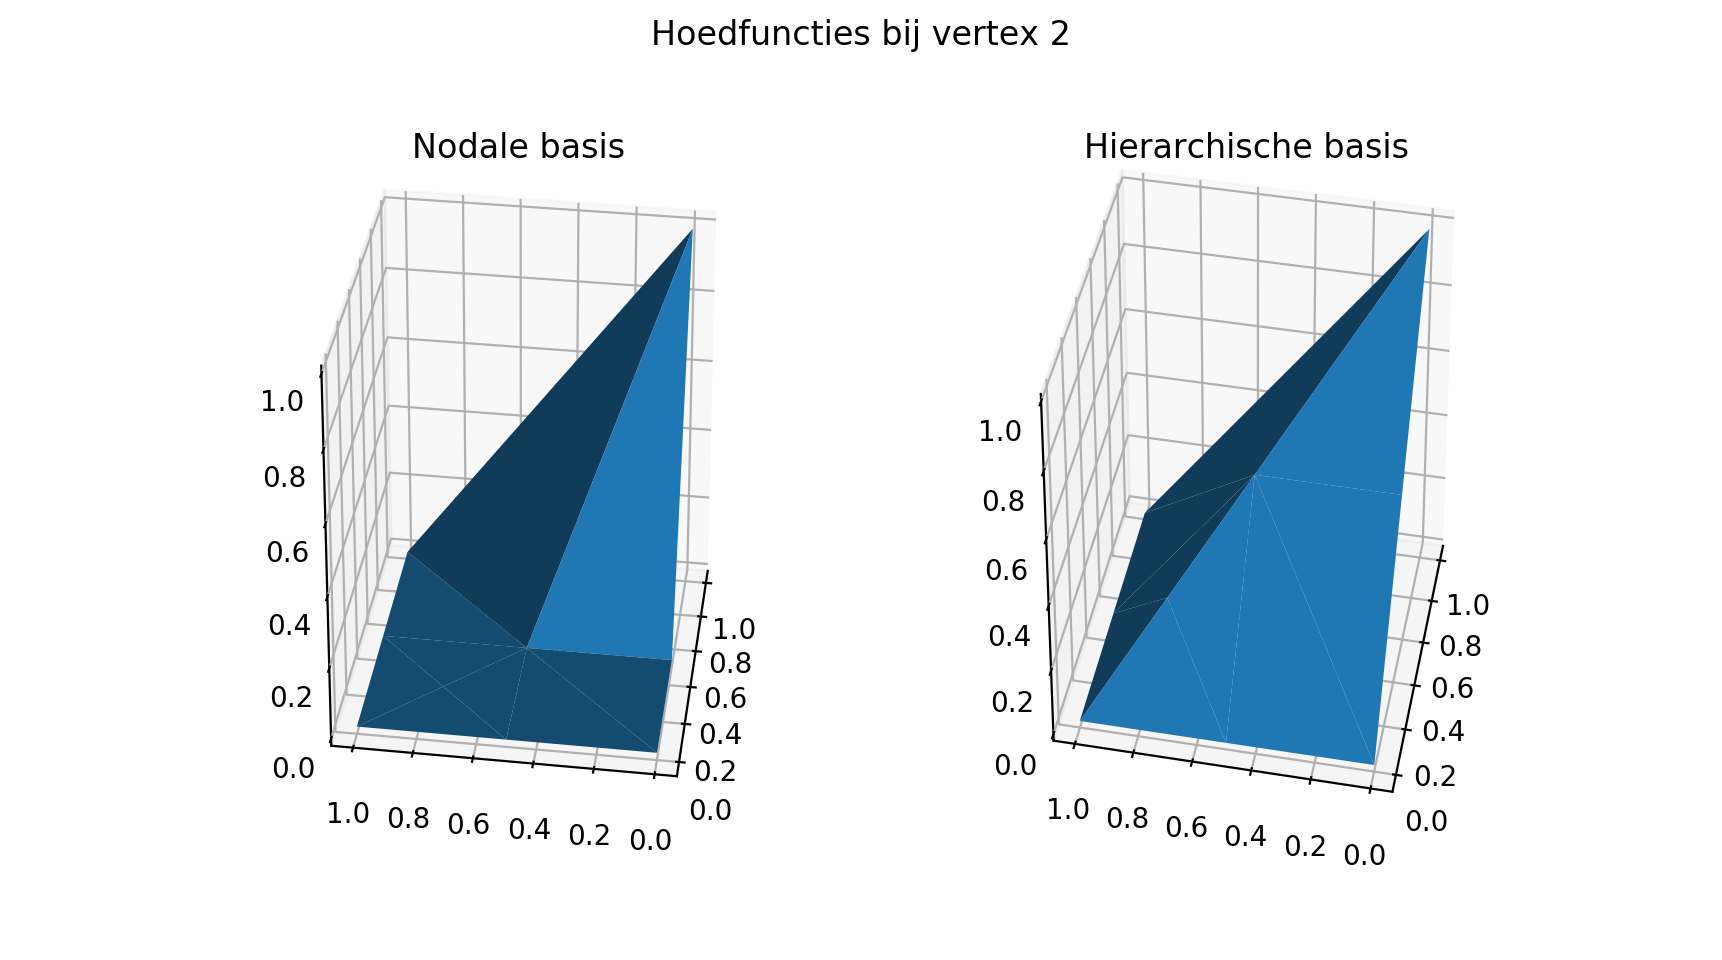
\includegraphics[width=\linewidth]{img/h2.png}\\
    \vspace{-2em}
  \end{minipage}
  \caption{Links: De bijbehorende vertex family-tree. Rechts: De functies $\psi_i$ en $\phi_i$ voor $i=0,2$---gebouwd dmv $\T_5$\texttt{.applyT(e\_i)}.}
\end{figure}


\end{document}
